\documentclass[a4paper, 12pt]{article}
\usepackage{graphicx}
\usepackage[margin=1in]{geometry}
\usepackage{titlesec}
\usepackage{indentfirst}
\usepackage{setspace}
\usepackage{amsmath}
\usepackage{amssymb}
\usepackage[outputdir = ../]{minted}
\usepackage[svgnames]{xcolor}
\usepackage[hidelinks]{hyperref}
\usepackage{tabularray}
\usepackage{graphbox}
\usepackage{float}
\usepackage{comment}
\usepackage{longtable,booktabs,array}
\usepackage{calc}
\usepackage{subfig}
\usepackage[
    backend=biber,
    style=authoryear,
  ]{biblatex}
\addbibresource{bib.bib}

\titleformat{\section}[block]{\large\bfseries}{\thesection}{0.5cm}{}
\titleformat{\subsection}[block]{\normalfont\bfseries}{\thesubsection}{0.5cm}{}
\titlespacing{\subsection}{8pt}{8pt}{8pt}

\newcommand\mefvm{%
    \textit{m}\kern-.1em%
    \raise0.5ex\hbox{\textit{e}}\kern-.1em%
    \textit{f}\kern-.2em%
    \raise-0.5ex\hbox{\textit{v}}\kern-.05em%
    \textit{m}
}
\renewcommand{\labelitemi}{-}
\renewcommand{\labelitemii}{-}

\begin{document}
\doublespacing
\begin{titlepage}
    \begin{center}
        
\includegraphics[width=0.8\textwidth]{HW3/university1.pdf}\\
        
        \textbf{ME485: Computational Fluid Dynamics \\ Using Finite Volume Method}

        \vspace{0.5cm}
        Homework 3
            
        \vspace{1.5cm}

        \textbf{Uğur Ozan Baygeldi}\\
        \textbf{Ali Kaya}\\ 
        \textbf{Onur Kakilli}\\~\\
        Group 15
        
    \end{center}
\end{titlepage}

\section{Introduction}

This report is on the second homework of the course ME485, Computational Fluid Dynamics Using Finite Volume Method. The homework requests integration of limiters and upwinding methods to \mefvm\!. \nocite{gi} \nocite{hw1} \nocite{hw2}

\section{Roadmap}
This homework has an extra step to implement unlike other two completed beforehand. The extra task is to implement a feature called "Barth-Jespersen limiter" which is generally used in highly turbulent, supersonic, or even hypersonic applications to record flow or shock properties in high definitions. The Homework requires to implement:

\begin{itemize}
    \item Implement \verb|_make_compute_norm|, \verb|_make_compute_fpts| and \\\verb|_make_barth_jespersen| to \verb|AdvectionElements| class at \verb|elements.py|
    
    \item Implement \verb|make_minmax| to \verb|AdvectionIntInters| and \verb|AdvectionBCInters| classes at \verb|inters.py|
    
    \item Implement \verb|make_flux| to \verb|AdvectionIntInters| and \verb|AdvectionBCInters| classes at \verb|inters.py|
    
    \item Implement \verb|upwind| and \verb|Local-Lax-Friedrich (Rusanov) flux functions| to \\\verb|AdvectionIntInters| at \verb|fsolver.py|
\end{itemize} \par

Following the same methodology used in the previous two homework the roadmap was implemented according to the order called at \verb|system.py|. Using this method also allows for checking memory errors by printing the word here occasionally after certain steps. \\\par
Furthermore, this homework requires checking different conditions over different meshes which is done by implementing different equations and creating different meshes using \verb|gmsh|.

\section{Implementation of \texttt{\_make\_compute\_fpts} and \texttt{\_make\_barth\_jespersen} at \texttt{elements.py}}
\subsection{Implementation of \texttt{\_make\_compute\_fpts}}

The implementation of \verb|_make_compute_fpts| is done easily after numerous implementations in homeworks 1 and 2. The code simply assigns the cell center values of elements for the given function to faces.\\\par

To implement this function the following code is utilized:
\begin{minted}[frame=lines,framesep=2mm,baselinestretch=1.2,bgcolor=Cornsilk,fontsize=\footnotesize,linenos]{python}
    def _make_compute_fpts(self):
        nvars, nface = self.nvars, self.nface
        def _compute_fpts(i_begin, i_end, upts, fpts):
            # Code taken directly from HW1
            for idx in range(i_begin, i_end):
                for j in range(nvars):
                    for i in range(nface):
                        fpts[i, j, idx] = upts[j, idx]
        return self.be.make_loop(self.neles, _compute_fpts)
\end{minted}

\subsection{Implementation of \texttt{\_make\_barth\_jespersen}}
Barth-Jespersen limiter is a commonly used limiter in the world of CFD. A limiter is used to prevent non-physical results rising from oscillations from appearing in the simulations.

\subsubsection{Mathematical Implementation of \texttt{\_make\_barth\_jespersen}}

The Barth-Jespersen limiter is simply the following. (\cite{lect})

\begin{equation}
\Psi_0 = \min_f 
\begin{cases} 
\min \left(1, \frac{\phi_{\text{max}} - \phi_0}{\Delta_f} \right) & \text{if } \Delta_f > 0, \\
\min \left(1, \frac{\phi_{\text{min}} - \phi_0}{\Delta_f} \right) & \text{if } \Delta_f < 0, \\
1 & \text{if } \Delta_f = 0,
\end{cases}
\end{equation} \par

Where:
\begin{itemize}
    \item $\phi_{\text{max}}$ and $\phi_{\text{min}}$ are the maximum and minimum values of $\phi$ in the stencil.
    \item $\phi_0$ is the current cell value.
    \item $\Delta_f = \nabla q_0 \cdot \mathbf{r}_{0,f}$ is the change in the unlimited reconstructed values at the face.
\end{itemize}

\subsubsection{Code Implementation of \texttt{\_make\_barth\_jespersen}}
The Barth-Jespersen limiter is implemented in the code using the following statements:

\begin{minted}[frame=lines,framesep=2mm,baselinestretch=1.2,bgcolor=Cornsilk,fontsize=\footnotesize,linenos]{python}
    def _make_barth_jespersen(self, limiter):
        nface, ndims,  nvars = self.nface, self.ndims, self.nvars
        dxf = self.dxf
        # Compiler arguments
        array = self.be.local_array()
        
        def _cal_barth_jespersen(i_begin, i_end, upts, grad, fext, lim):
            for i in range(i_begin, i_end):
                for j in range(nvars):
                    fiList = np.zeros(nface)
                    fiMax = max(fext[0, :, j, i])
                    fiMin = min(fext[1, :, j, i])
                    for f in range(nface):
                        deltaF = dot(grad[:, j, i], dxf[f, :, i], ndims) + eps
                        if   deltaF > 0:
                            fiList[f] = min(1,(fiMax - upts[j, i])/deltaF)
                        elif deltaF < 0:
                            fiList[f] = min(1,(fiMin - upts[j, i])/deltaF)
                        elif deltaF == 0:
                            fiList[f] = 1
                    lim[j, i] = min(fiList)
        return self.be.make_loop(self.neles, _cal_barth_jespersen)
\end{minted} 
\par

The code implements what was stated in the mathematical expressions. First checks the delta F value and then determines the limits. \\\par

After the limits are determined, the \verb|lim| array is filled appropriately to be used further in the flux calculations.

\section{Implementation of \texttt{\_make\_minmax}} \label{c4} 

The function \verb|_make_minmax| is used to determine the maximum and minimum of neighboring cell faces. The function then simply assigns the max and min to the specified position in the \verb|fext| array.

\subsection{Code Implementation of \texttt{\_make\_minmax}} 

The following code implements the method. Note that for the below code the array name is \verb|uext|, which will be used as the \verb|fext| array mentioned in \hyperref[c4]{\textit{chapter 4}}

\begin{minted}[frame=lines,framesep=2mm,baselinestretch=1.2,bgcolor=Cornsilk,fontsize=\footnotesize,linenos]{python}
    def _make_minmax(self):
        nvars = self.nvars
        lt, le, lf = self._lidx
        rt, re, rf = self._ridx

        def compute_minmax(i_begin, i_end, uf, *uext):
            for idx in range(i_begin, i_end):
                lti, lfi, lei = lt[idx], lf[idx], le[idx]
                rti, rfi, rei = rt[idx], rf[idx], re[idx]

                for j in range(nvars):
                    ul = uf[lti][lfi, j, lei]
                    ur = uf[rti][rfi, j, rei]

                    uext[lti][0, lfi, j, lei] = max(ul, ur)
                    uext[lti][1, lfi, j, lei] = min(ul, ur)

                    uext[rti][0, rfi, j, rei] = max(ul, ur)
                    uext[rti][1, rfi, j, rei] = min(ul, ur)

        return self.be.make_loop(self.nfpts, compute_minmax)
\end{minted}
\par
Similarly, the \verb|bc| function is required to adjust the "ghost elements" neighboring the boundary element for the \verb|AdvectionBCInters| class. \\\par

However, for the boundary case, since there is no right element, there is no setting of the right element position at \verb|uext|.\\\par

The code for the boundary elements are as follows:
\begin{minted}[frame=lines,framesep=2mm,baselinestretch=1.2,bgcolor=Cornsilk,fontsize=\footnotesize,linenos]{python}
    def _make_minmax(self):
        nvars = self.nvars
        ndims = self.ndims
        lt, le, lf = self._lidx
        nf = self._vec_snorm

        bc = self.bc
        array = self.be.local_array()

        def compute_minmax(i_begin, i_end, uf, *uext):

            for idx in range(i_begin, i_end):
                lti, lfi, lei = lt[idx], lf[idx], le[idx]
                ur = array(nvars)
                vr = array(ndims)
                vl = array(ndims)

                ul = uf[lti][lfi, :, lei]
                bc(ul, ur, vl, vr, nf[:, idx])

                for j in range(nvars):

                    uext[lti][0, lfi, j, lei] = max(ul[j], ur[j])
                    uext[lti][1, lfi, j, lei] = min(ul[j], ur[j])

        return self.be.make_loop(self.nfpts, compute_minmax)
\end{minted}

\section{Implementation of \texttt{\_make\_flux}}

The purpose of setting limiters and calculating gradients is to obtain the flux values. This section of the code ties everything together yielding a sensible result.

\subsection{Code Implementation of \texttt{\_make\_flux}} 

To implement \verb|_make_flux| for the \verb|AdvectionIntInters| the following code is utilized. This function is similar to a case for the actual flux schemes. \\\par 

A \hyperref[bcf]{\textit{similar code}} will be used for the \verb|AdvectionBCInters| which will be explained later: \\\par

\begin{minted}[frame=lines,framesep=2mm,baselinestretch=1.2,bgcolor=Cornsilk,fontsize=\footnotesize,linenos]{python}
    def _make_flux(self):
        ndims, nfvars = self.ndims, self.nfvars
        lt, le, lf = self._lidx
        rt, re, rf = self._ridx
        nf, sf = self._vec_snorm, self._mag_snorm
        # Compiler arguments
        array = self.be.local_array()
        cplargs = {
            'flux_func' : self.ele0.flux_container(),
            'ndims' : ndims,
            'nfvars' : nfvars,
            'array' : array,
            **self._const
        }

        # Get numerical schems from `rsolvers.py`
        scheme = self.cfg.get('solver', 'flux')
        flux = get_fsolver(scheme, self.be, cplargs)

        def comm_flux(i_begin, i_end, vf, *uf):
            for idx in range(i_begin, i_end):
                # flux function to be filled
                fn = array(nfvars)
                lti, lfi, lei = lt[idx], lf[idx], le[idx]
                rti, rfi, rei = rt[idx], rf[idx], re[idx]
                nfi = nf[:, idx]

                ul = uf[lti][lfi, :, lei]
                ur = uf[rti][rfi, :, rei]

                vl = vf[lti][lfi, :, lei]
                vr = vf[rti][rfi, :, rei]

                # call the numerical flux function here : i.e. upwind or rusanov
                flux(ul, ur, vl, vr, nfi, fn)

                for jdx in range(nfvars):
                    # Save it at left and right solution array
                    uf[lti][lfi, jdx, lei] =  fn[jdx]*sf[idx]
                    uf[rti][rfi, jdx, rei] = -fn[jdx]*sf[idx]

        return self.be.make_loop(self.nfpts, comm_flux)
\end{minted}
\par

\mefvm computes the different flux schemes separately in a file called \verb|fsolvers.py| which will be further explained in \hyperref[c6]{\textit{chapter 6}}. The code takes the required arguments and feeds them to the flux function. Which also has the scheme info. (lines 17 \& 18) \\\par

For the \verb|AdvectionBCInters|, similar to \verb|_make_minmax| the \verb|bc| function is called. 

\begin{figure}[H]
\begin{minted}[frame=lines,framesep=2mm,baselinestretch=1.2,bgcolor=Cornsilk,fontsize=\footnotesize,linenos]{python}
    def _make_flux(self, nele):
        ndims, nfvars = self.ndims, self.nfvars
        lt, le, lf = self._lidx
        nf, sf = self._vec_snorm, self._mag_snorm
        
        # Compiler arguments
        array = self.be.local_array()
        cplargs = {
            'flux_func' : self.ele0.flux_container(),
            'ndims' : ndims,
            'nfvars' : nfvars,
            'array' : array,
            **self._const
        }

        # Get numerical schems from `rsolvers.py`
        scheme = self.cfg.get('solver', 'flux')
        flux = get_fsolver(scheme, self.be, cplargs)
        # Get bc function 
        bc = self.bc

        def comm_flux(i_begin, i_end, vf, *uf):

            for idx in range(i_begin, i_end):
                fn = array(nfvars)

                lti, lfi, lei = lt[idx], lf[idx], le[idx]
                nfi = nf[:, idx]
                ul = uf[lti][lfi, :, lei]
                vl = vf[lti][lfi, :, lei]
                vr = array(ndims)
                ur = array(nfvars)
                bc(ul,ur,vl,vr,nfi)

                flux(ul, ur, vl, vr, nfi, fn)

                for jdx in range(nfvars):
                    # Save it at left solution array
                    uf[lti][lfi, jdx, lei] = fn[jdx]*sf[idx]

        return self.be.make_loop(self.nfpts, comm_flux)
\end{minted} 
\label{bcf}
\end{figure}
\par

\section{Implementation of \texttt{Upwind} and \texttt{Local-Lax-Friedrich (Rusanov)}} \label{c6}

\verb|Upwind| and \verb|Local-Lax-Friedrich (Rusanov)| are both flux schemes used commonly. Both of these schemes have strong sides and weak sides.

\subsection{Mathematical Implementation of \texttt{Upwind}}
The upwind flux determines the flux based on the direction of the velocity field:
\begin{equation}
F_{\text{upwind}} = 
\begin{cases} 
\mathbf{v} \phi_{\text{upwind}} & \text{if } \mathbf{v} \cdot \mathbf{n} > 0, \\
\mathbf{v} \phi_{\text{downwind}} & \text{if } \mathbf{v} \cdot \mathbf{n} \leq 0,
\end{cases}
\end{equation}
\begin{itemize}
    \item $\phi_{\text{upwind}}$ is the value of $\phi$ in the upstream direction (where the flow originates).
    \item $\phi_{\text{downwind}}$ is the value of $\phi$ in the downstream direction (where the flow exits).
\end{itemize} \par

This method ensures stability by using information from the direction of incoming flow.

\subsection{Code Implementation of \texttt{Upwind}}
The main implementation of the flux schemes relies on the \verb|flux_func| argument taken from the \verb|advection.ini| file. Where the code parses the equation to be machine-readable. \\\par
The code to implement \verb|Upwind| relies on the dot product of vectors to determine the flow direction after that the flux at the interface can be selected which can be simply implemented using the following block:

\begin{minted}[frame=lines,framesep=2mm,baselinestretch=1.2,bgcolor=Cornsilk,fontsize=\footnotesize,linenos]{python}
def make_upwind(cplargs):
    nvars     = cplargs['nfvars']
    gamma     = cplargs['gamma']
    flux_func = cplargs['flux_func']
    array     = cplargs['array']
    ndims     = cplargs['ndims']
    def fsolver(ul, ur, vl, vr, nf, fn):
    
        fl = array(nvars)
        fr = array(nvars)
        flux_func(ul, vl, nf, fl)
        flux_func(ur, vr, nf, fr)
        
        if dot(vl, nf, ndims) > 0:
            for i in range(nvars):
                fn[i] = fl[i]
        else:
            for i in range(nvars):
                fn[i] = fr[I]
                
    return fsolver
\end{minted}

\subsection{Mathematical Implementation of \texttt{Local-Lax-Friedrich (Rusanov)} flux}

The Local Lax-Friedrichs flux, also known as the Rusanov flux, provides a balance between stability and accuracy by incorporating both the central flux and a dissipation term. It is expressed as: \label{sec:rusanov}

\begin{equation}
F_{\text{Rusanov}} = \frac{1}{2} \left[ \mathbf{v} (\phi_{\text{left}} + \phi_{\text{right}}) - |\lambda| (\phi_{\text{right}} - \phi_{\text{left}}) \right]
\end{equation} \par

Here:
\begin{itemize}
    \item $\phi_{\text{left}}$ and $\phi_{\text{right}}$ are the values of $\phi$ on the left and right sides of the interface, respectively. These represent the reconstructed values from adjacent cells.
    \item $|\lambda|$ is the spectral radius (or the maximum eigenvalue) of the Jacobian matrix of the flux function. In the case of advection, $|\lambda|$ corresponds to the maximum magnitude of the velocity, $|\mathbf{v}|$, across the interface.
\end{itemize} \par

The Rusanov flux can be understood in two parts:
\begin{enumerate}
    \item \textbf{Central Flux:} The term $\mathbf{v} (\phi_{\text{left}} + \phi_{\text{right}})$ computes the average flux contribution from both sides of the interface. This ensures a symmetric treatment of the interface.
    \item \textbf{Dissipation Term:} The term $-|\lambda| (\phi_{\text{right}} - \phi_{\text{left}})$ introduces numerical dissipation, which stabilizes the solution by dampening oscillations or discontinuities at the interface.
\end{enumerate}

The balance between these two components allows the Rusanov flux to handle sharp gradients and discontinuities in $\phi$ while maintaining numerical stability. This makes it particularly effective for solving hyperbolic equations such as the advection equation.
\subsection{Code Implementation of \texttt{Local-Lax-Friedrich (Rusanov)} flux}
To implement \verb|Local-Lax-Friedrich (Rusanov)| flux the following code is used. 
\begin{minted}[frame=lines,framesep=2mm,baselinestretch=1.2,bgcolor=Cornsilk,fontsize=\footnotesize,linenos]{python}
def make_rusanov(cplargs):
    nvars     = cplargs['nfvars']
    gamma     = cplargs['gamma']
    flux_func = cplargs['flux_func']
    array     = cplargs['array']
    ndims     = cplargs['ndims']
    def fsolver(ul, ur, vl, vr, nf, fn):
        fl = array(nvars)
        fr = array(nvars)

        # this is u*phi*n 
        flux_func(ul, vl, nf, fl)
        flux_func(ur, vr, nf, fr)
        a = max(abs(dot(vl, nf, ndims)), abs(dot(vr, nf, ndims)))

        for i in range(nvars):
            fn[i] = 0.5 * (fl[i] + fr[i]) - 0.5 * a * (ur[i] - ul[i])

    return fsolver
\end{minted}

The $\lambda$ value mentioned in \hyperref[sec:rusanov]{\textit{section 6.3}} is calculated by comparing absolute values of the velocities of the elements normal to the face and picking the maximum. After which the Rusanov scheme is used.

\section{Implementation of \texttt{\_make\_compute\_norm}}

This homework requires the area to be calculated which will be taken as the norm. To actually calculate the norm first calculated area is subtracted from the last area.

\subsection{Mathematical Implementation of \texttt{\_make\_compute\_norm}}

To implement \verb|_make_compute_norm| for this homework, there is no need for the exact solution. Essentially, the sum of all the element volumes with $\phi \leq 0$.

\subsection{Code Implementation of \texttt{\_make\_compute\_norm}}

The code to implement the requested norm uses the array \verb|upts|, note that the index 0 of the array is used. This index houses the $\phi$ values. With an if statement the element is checked to see if it satisfies the condition. If it does the volume of the element is added to the total.  \\\par

The code to implement \verb|_make_compute_norm| is as follows:

\begin{minted}[frame=lines,framesep=2mm,baselinestretch=1.2,bgcolor=Cornsilk,fontsize=\footnotesize,linenos]{python}
    def _make_compute_norm(self):
        import numba as nb
        vol = self._vol
        neles, nvars, ndims = self.neles, self.nvars, self.ndims
        xc = self.xc.T   
        def run(upts):
            norm = np.zeros(nvars)
            for i in range(neles):
                for j in range(nvars):
                    if upts[0][j, i] <= 0:
                        norm[j] += vol[i]
            return norm

        return self.be.compile(run, outer=True)
\end{minted}


\section{Tests and Results}

In this part of the report, tests of various geometries with different mesh structures (triangular/quadrilateral, structured/unstructured); different test cases by changing level set functions and velocity profiles; different numeric flux calculation methods, and lastly with varying steps of time will be conducted to see the boundaries of the code implemented.\\\par

All the results will be tabulated for easier viewing and commenting. Furthermore, you can visit \href{https://www.baygeldi.com/485_2}{\textbf{here}} to see the output.

\subsection{Meshes}
A table explaining all the meshes, with node and element counts, will be provided in the \hyperref[ap]{\textit{appendix}} \\\par

The first mesh tested is already provided within the homework code (\cite{gi}). As seen from the figure below, it consists of a rectangle divided into two equal parts. Although they are symmetric, each side has a different mesh type. While one side contains quadrilateral mesh elements, the other contains triangular-type elements. Moreover, the quadrilateral side is also more structured than the triangle side. This creates a test for the interface between quadrilateral and triangular mesh types, allowing to check for any numerical errors.

%1740 nodes 2782 elements
\begin{figure}[h]
    \centering
    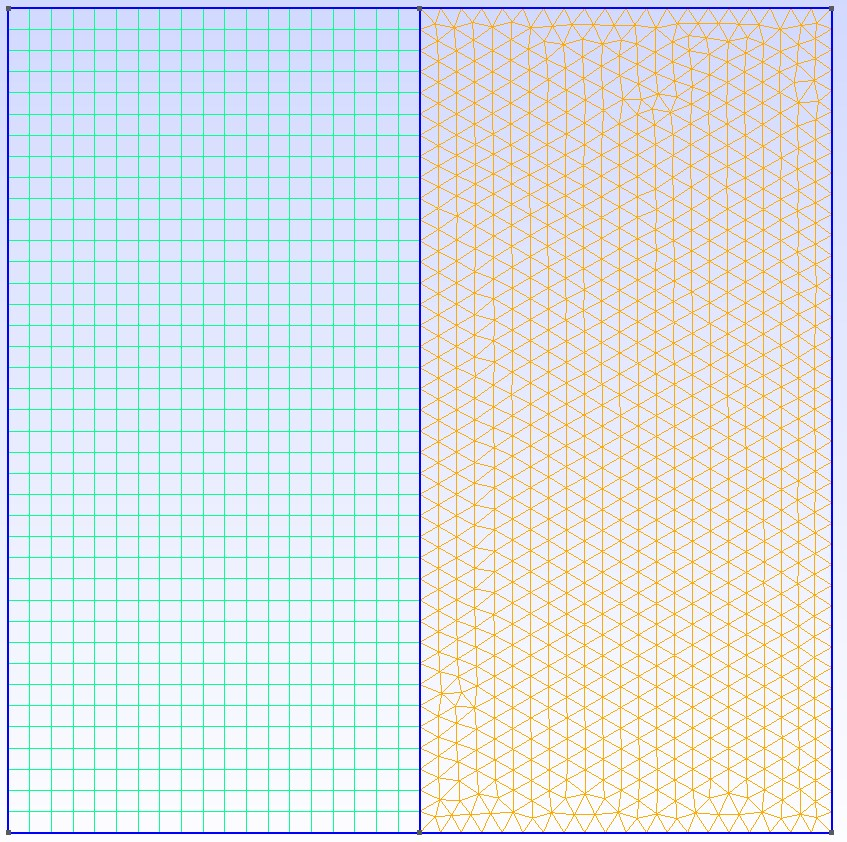
\includegraphics[width=0.4\linewidth]{HW3/Test Mesh Provided.jpg}
    \caption{Provided Test Mesh Geometry}
\end{figure}\par

The second test mesh is constructed to see the effect of "division" number of main geometry. It is also seasoned with two structural quadrilateral elements and two unstructured triangular elements. In this mesh, more transitions between the element shapes are observed. This mesh has 3 interface sides with different element types which is 2 more than the first mesh. \\\par The mesh can be seen on the next page.

%???? nodes ???? elements
\begin{figure}[H]
    \centering
    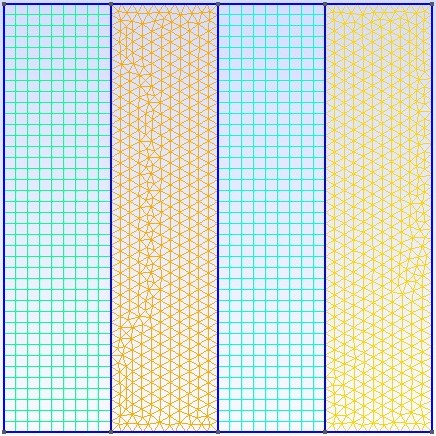
\includegraphics[width=0.4\linewidth]{HW3/2Structured2furious.jpg}
    \caption{Four Section Structured/Unstructured Test Mesh Geometry}
\end{figure}\par

The third mesh is a purely triangular mesh which will be used along the fourth mesh to check whether quadrilateral or triangular elements are better. These two meshes will also help compare the different velocity fields. \\\par

The third mesh is as follows:

\begin{figure}[H]
    \centering
    
\includegraphics[width=0.4\linewidth]{HW3/minikt.jpeg}
    \caption{Triangular Element Test Mesh Geometry}
\end{figure}\par

Similarly, the fourth mesh is a fully quadrilateral mesh with relative fineness to the triangular one. \\\par

The fourth mesh can be seen on the next page.

\begin{figure}[H]
    \centering
    
\includegraphics[width=0.4\linewidth]{HW3/miniks.jpeg}
    \caption{Quadrilateral Element Test Mesh Geometry}
\end{figure}\par

\subsection{Velocity Fields}
To test the meshes, several different velocity fields have been created. \\\par

The first field is given by the instructor (\cite{gi}). Which creates a spiraling velocity field that does not mix the variable. This field can be expressed with the following expression:
\begin{equation*}
    u_x = -2\pi(y-0.5)\: \& \: u_y = 2\pi(x-0.5)
\end{equation*}
\vspace{-1cm}
\begin{figure}[h]
    \centering
    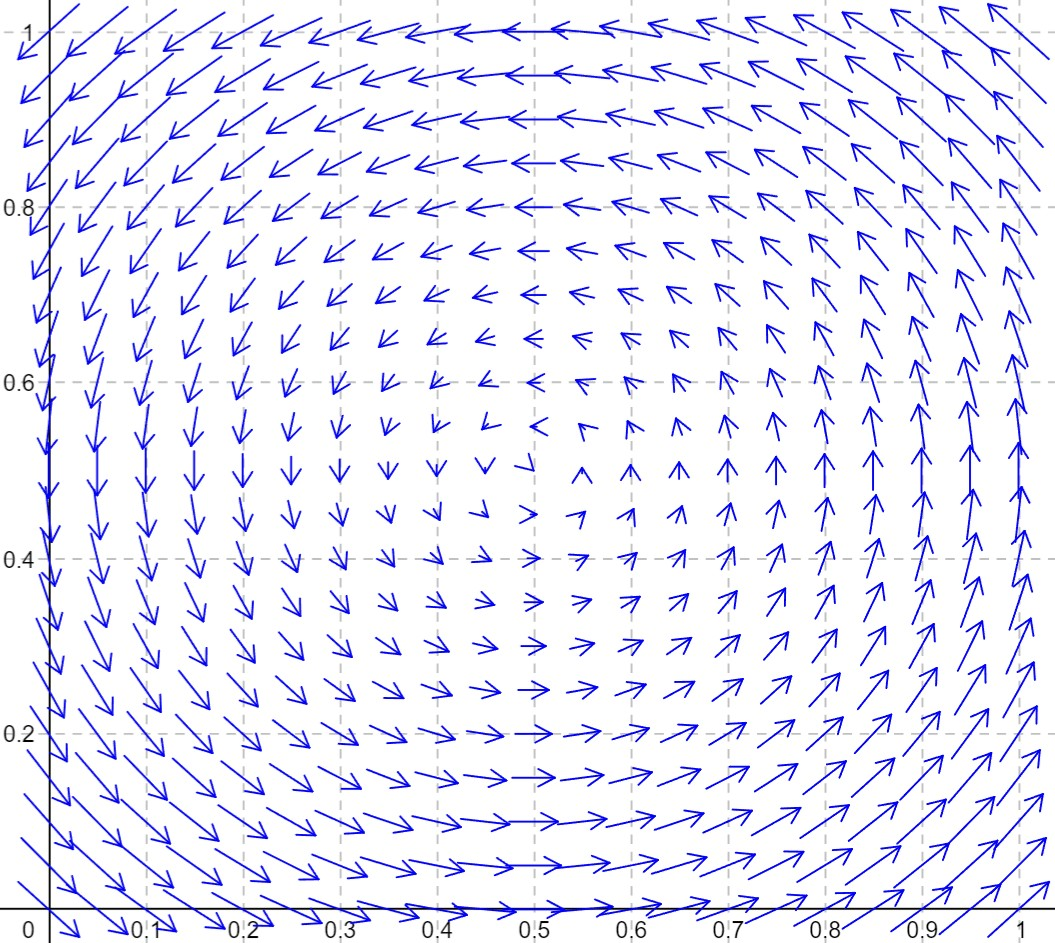
\includegraphics[width=0.35\linewidth]{HW3/default_vel.jpg}
    \caption{Provided Velocity Field (Field 1)}
    \label{f1}
\end{figure}\par

The second field is created to check the mixing of the field. This is done using the following expression:
\begin{equation*}
    u_x = sin(\pi x)cos(\pi y) \: \& \: u_y = -cos(\pi x)sin(\pi y)
\end{equation*}

\begin{figure}[h]
    \centering
    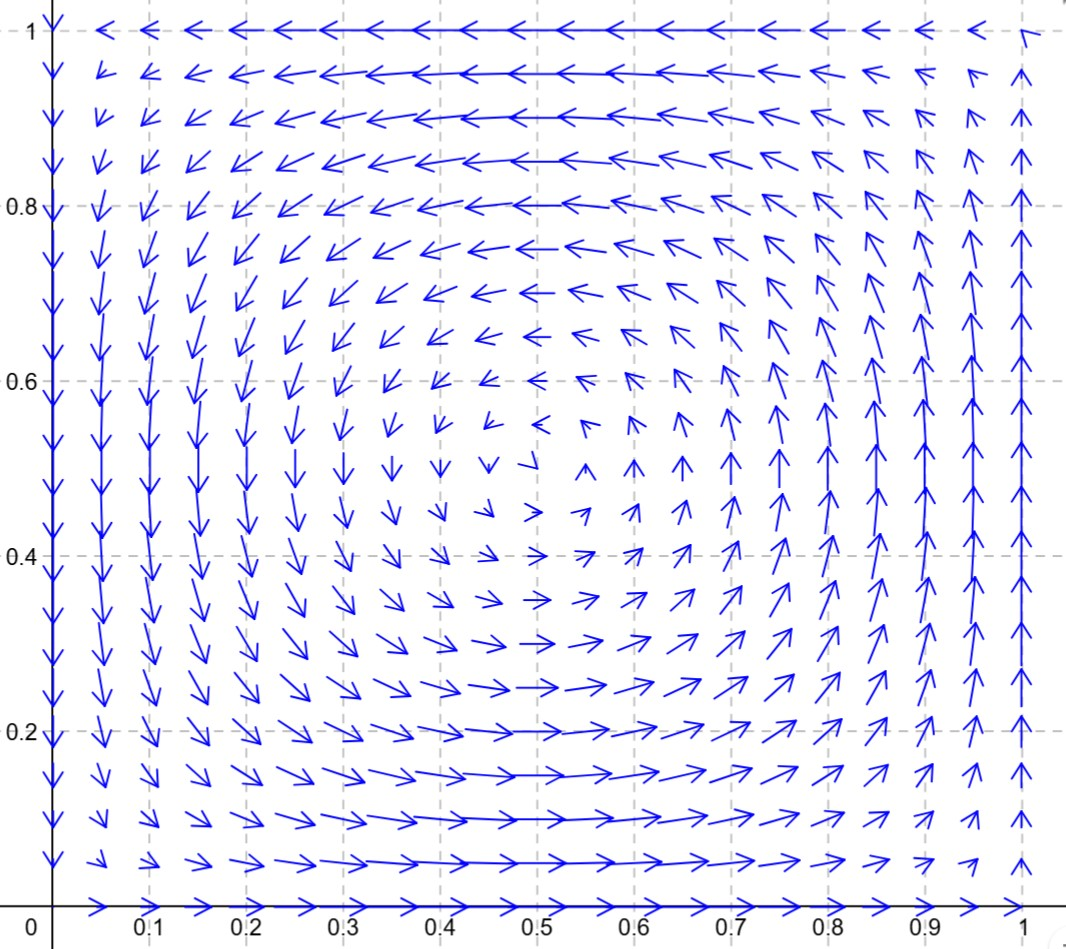
\includegraphics[width=0.35\linewidth]{HW3/vf2.jpeg}
    \caption{Mixing Velocity Field (Field 2)}
\end{figure}\par

The third field is pure advection towards the right. The velocity field is:
\begin{equation*}
    u_x = 0.3 \: \& \: u_y =0.0
\end{equation*}
\vspace{-1.5cm}
\begin{figure}[h]
    \centering
    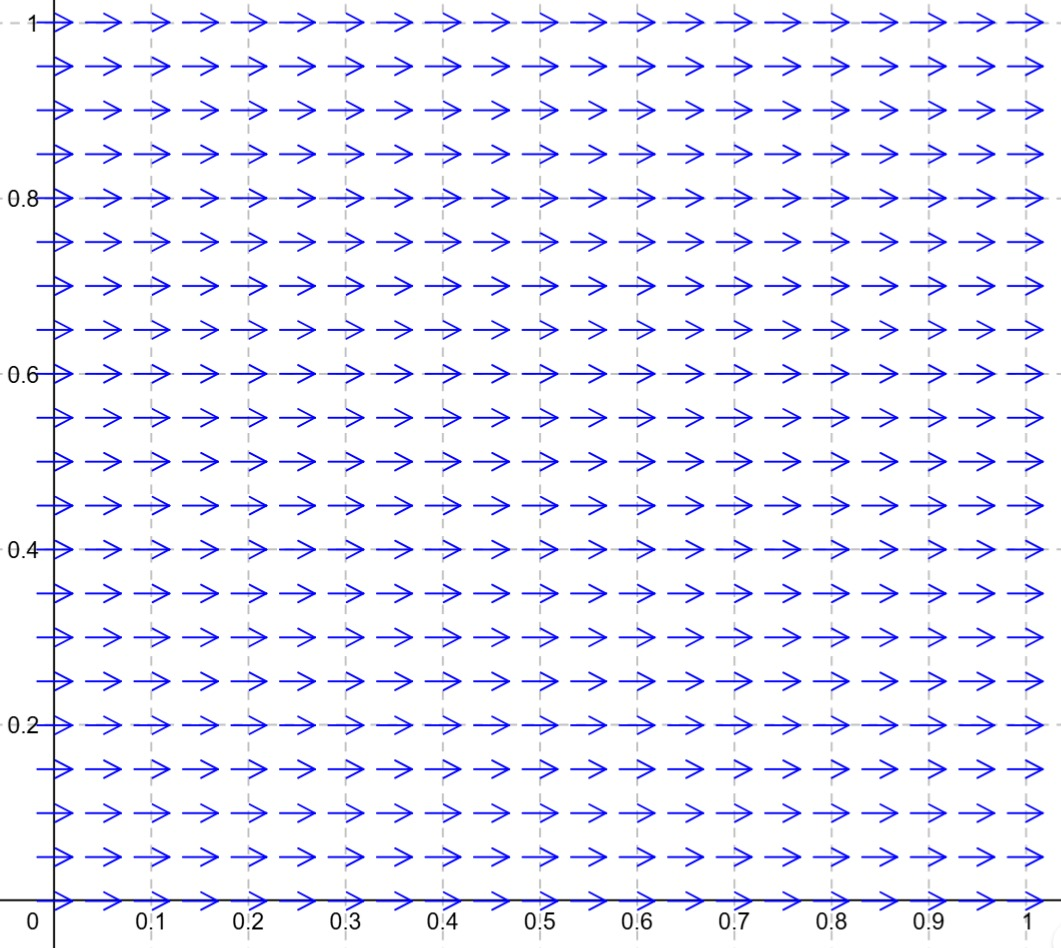
\includegraphics[width=0.35\linewidth]{HW3/vf3.jpeg}
    \caption{Advection to Right Velocity Field (Field 3)}
\end{figure}\par

The fourth velocity field has a discontinuity which prevents the calculations hence it will not be used. The field can be expressed as:
\begin{equation*}
    u_x = y-0.5 \: \& \: u_y = 0.0
\end{equation*}
\vspace{-1.5cm}
\begin{figure}[H]
    \centering
    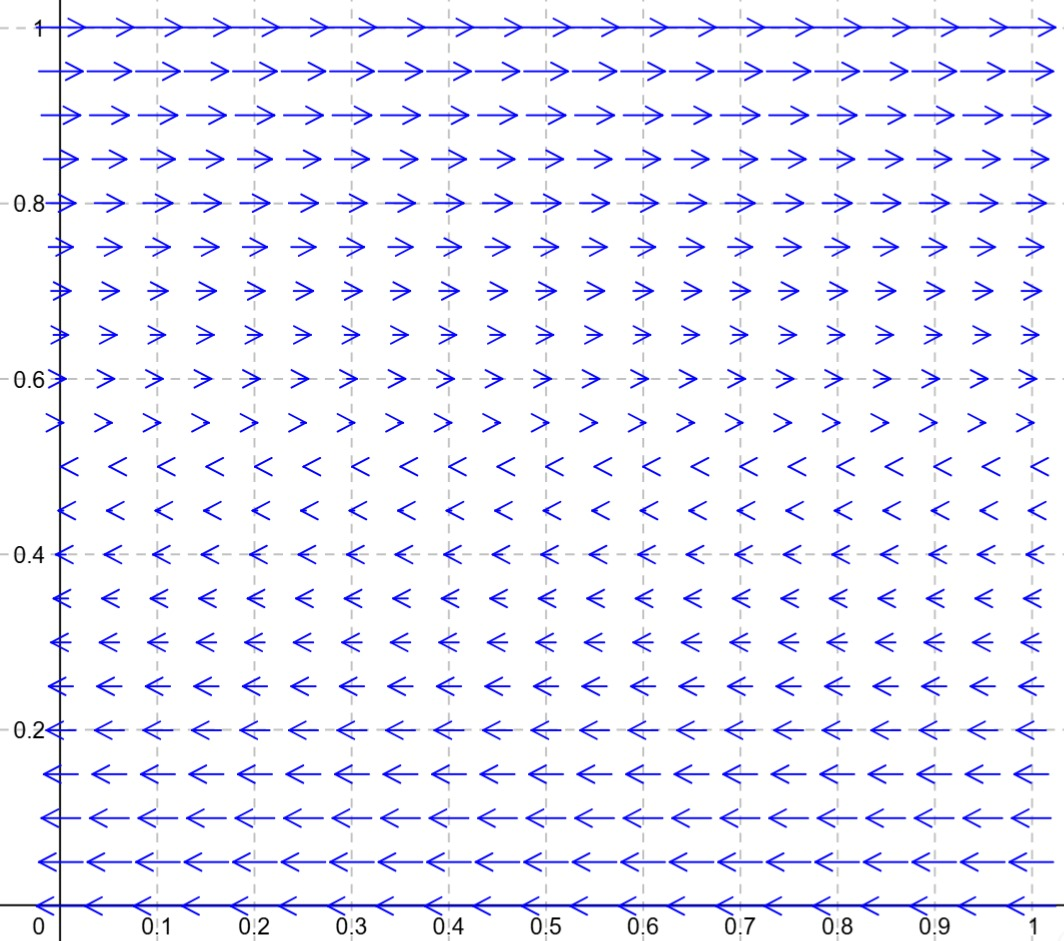
\includegraphics[width=0.35\linewidth]{HW3/vf4.jpeg}
    \caption{Discontinuous Velocity Field (Field 4)}
\end{figure}\par

These velocity fields are, again, tabulated at the \hyperref[ap2]{\textit{appendix}}.
\subsection{Obtained Norms}
The norms obtained for the different schemes using different meshes are as follows, refer to the caption to determine the functions.
\subsubsection{Timestep = 0.33}
\begin{table}[H]
    \renewcommand\baselinestretch{1.1}\selectfont
    \centering
    \mbox{}\clap{
    \begin{tblr}
        []{
        rowsep =1mm,
        colspec = {Q[c,m, 2cm]Q[c,m,4.7cm]Q[c,m,4.7cm]},
        vlines, hlines,
        row{1} = {gray9}
        }
        Mesh & Norm (Upwind) & Norm (Rusanov) \\
        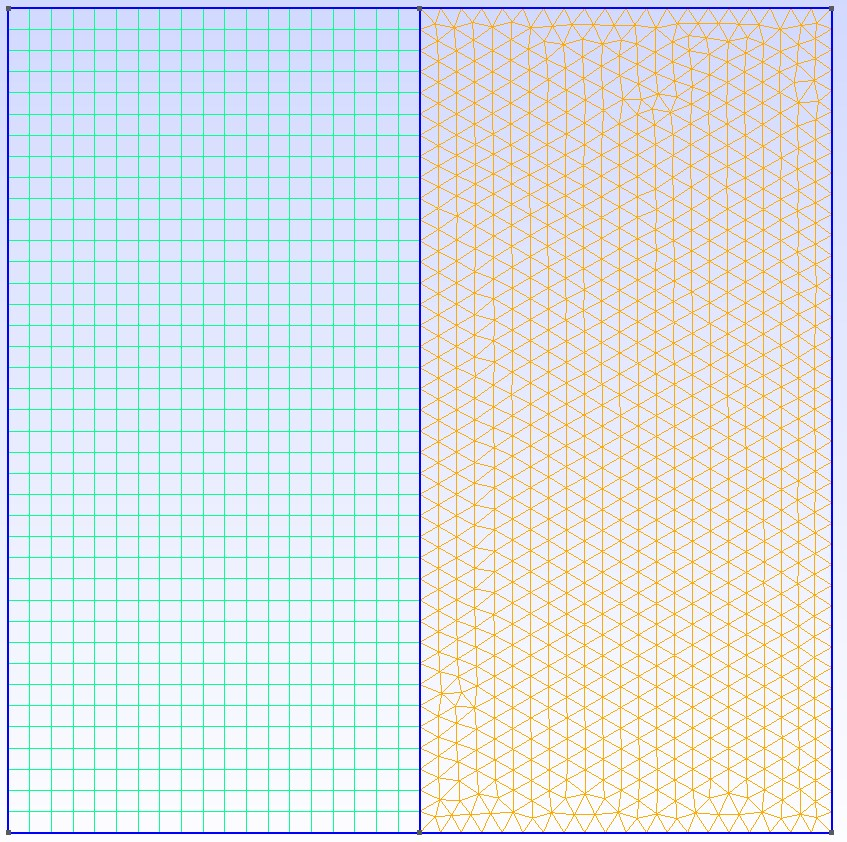
\includegraphics[width=0.4\linewidth, align=c]{HW3/Test Mesh Provided.jpg} Figure 1 & {[0.0018640]} & {[0.0018640]}\\
        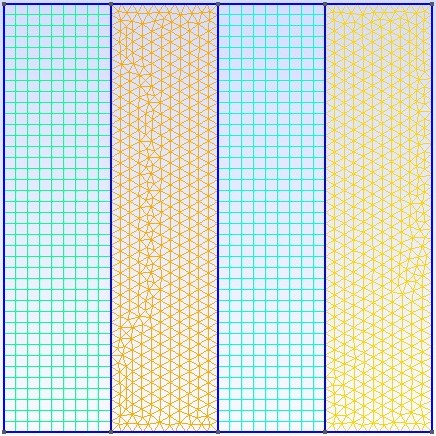
\includegraphics[width=0.4\linewidth, align=c]{HW3/2Structured2furious.jpg} Figure 2 & {[0,0073474]} & {[0.0073479]}\\
        
\includegraphics[width=0.4\linewidth, align=c]{HW3/minikt.jpeg} Figure 3 & {[0.0]} & {[0.0]}\\
        
\includegraphics[width=0.4\linewidth, align=c]{HW3/miniks.jpeg} Figure 4 & {[0.0001020]} & {[0.0001020]}\\
    \end{tblr}
    }
    \caption{Results for Given Function with Field 1 Dirichlet}
\end{table}
\begin{table}[H]
    \renewcommand\baselinestretch{1.1}\selectfont
    \centering
    \mbox{}\clap{
    \begin{tblr}
        []{
        rowsep =1mm,
        colspec = {Q[c,m, 2cm]Q[c,m,4.7cm]Q[c,m,4.7cm]},
        vlines, hlines,
        row{1} = {gray9}
        }
        Mesh & Norm (Upwind) & Norm (Rusanov) \\
        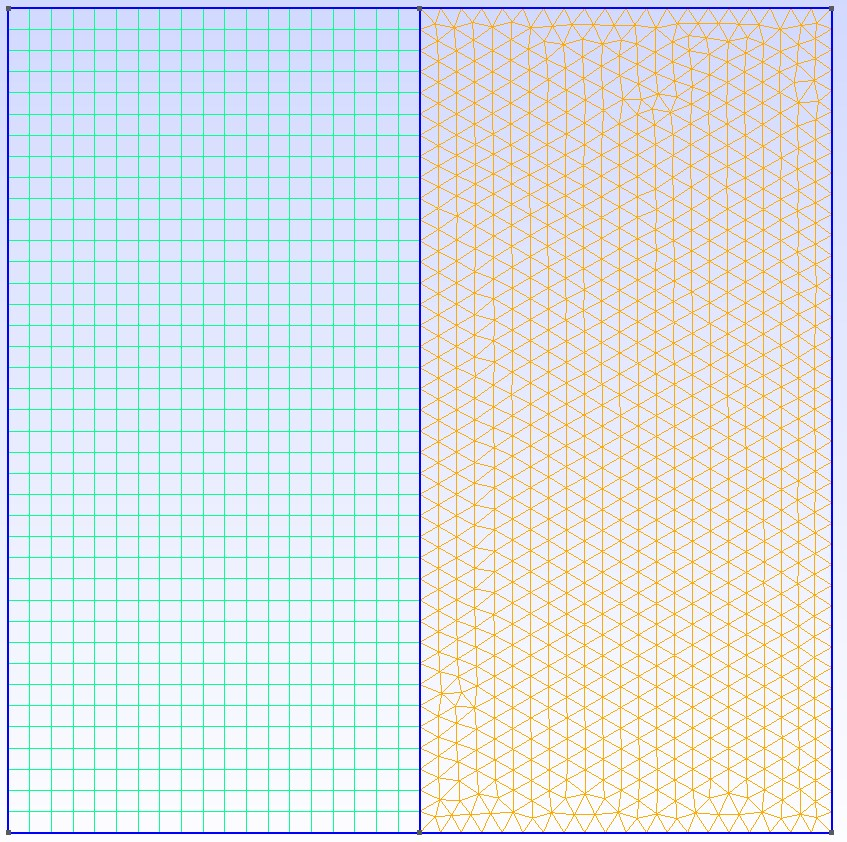
\includegraphics[width=0.4\linewidth, align=c]{HW3/Test Mesh Provided.jpg} Figure 1 & {[-0.0015359]} & {[-0.0015359]}\\
        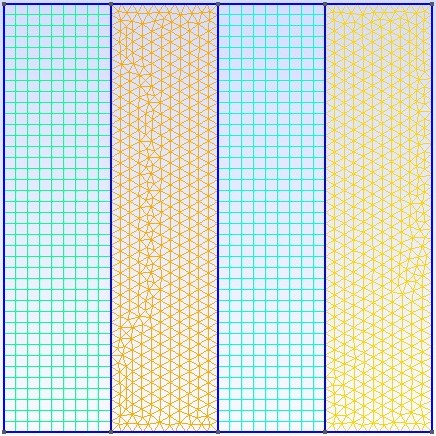
\includegraphics[width=0.4\linewidth, align=c]{HW3/2Structured2furious.jpg} Figure 2 & {[0.0195493]} & {[0.0195493]}\\
        
\includegraphics[width=0.4\linewidth, align=c]{HW3/minikt.jpeg} Figure 3 & {[-0.0005196]} & {[-0.0005196]}\\
        
\includegraphics[width=0.4\linewidth, align=c]{HW3/miniks.jpeg} Figure 4 & {[0.0]} & {[0.0]}\\
    \end{tblr}
    }
    \caption{Results for Given Function with Field 2 Dirichlet}
\end{table}
\begin{table}[H]
    \renewcommand\baselinestretch{1.1}\selectfont
    \centering
    \mbox{}\clap{
    \begin{tblr}
        []{
        rowsep =1mm,
        colspec = {Q[c,m, 2cm]Q[c,m,4.7cm]Q[c,m,4.7cm]},
        vlines, hlines,
        row{1} = {gray9}
        }
        Mesh & Norm (Upwind) & Norm (Rusanov) \\
        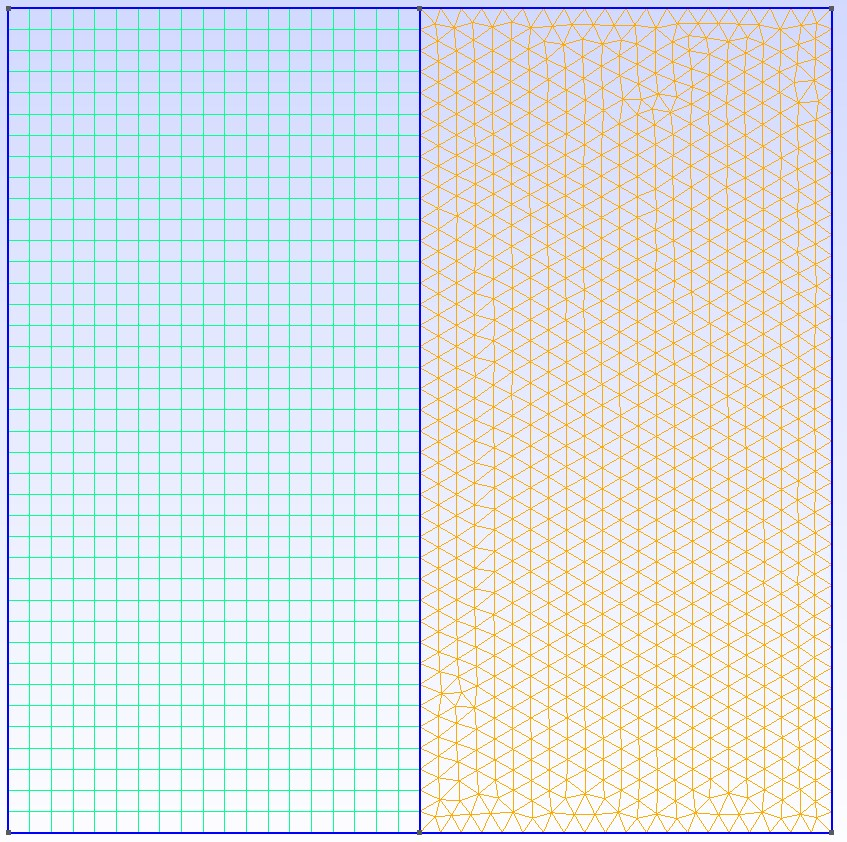
\includegraphics[width=0.4\linewidth, align=c]{HW3/Test Mesh Provided.jpg} Figure 1 & {[0.0092314]} & {[0.0092314]}\\
        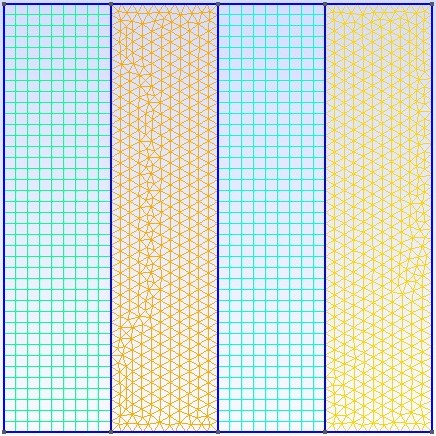
\includegraphics[width=0.4\linewidth, align=c]{HW3/2Structured2furious.jpg} Figure 2 & {[0.0212781]} & {[0.0212781]}\\
        
\includegraphics[width=0.4\linewidth, align=c]{HW3/minikt.jpeg} Figure 3 & {[0.0000127]} & {[0.0000127]}\\
        
\includegraphics[width=0.4\linewidth, align=c]{HW3/miniks.jpeg} Figure 4 & {[0.0007142]} & {[0.0007142]}\\
    \end{tblr}
    }
    \caption{Results for Given Function with Field 3 Dirichlet}
\end{table}
\vspace{-0.5cm}
\subsubsection{Timestep = 0.66}
\vspace{-0.5cm}
\begin{table}[H]
    \renewcommand\baselinestretch{1.1}\selectfont
    \centering
    \mbox{}\clap{
    \begin{tblr}
        []{
        rowsep =1mm,
        colspec = {Q[c,m, 2cm]Q[c,m,4.7cm]Q[c,m,4.7cm]},
        vlines, hlines,
        row{1} = {gray9}
        }
        Mesh & Norm (Upwind) & Norm (Rusanov) \\
        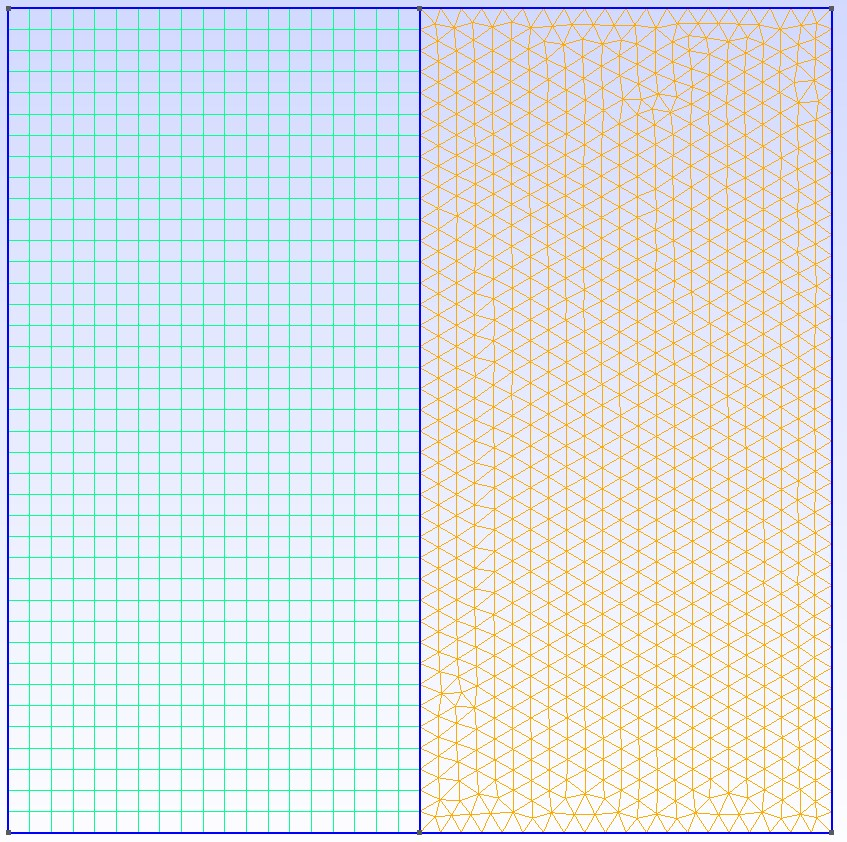
\includegraphics[width=0.4\linewidth, align=c]{HW3/Test Mesh Provided.jpg} Figure 1 & {[0.0054839]} & {[0.0054839]}\\
        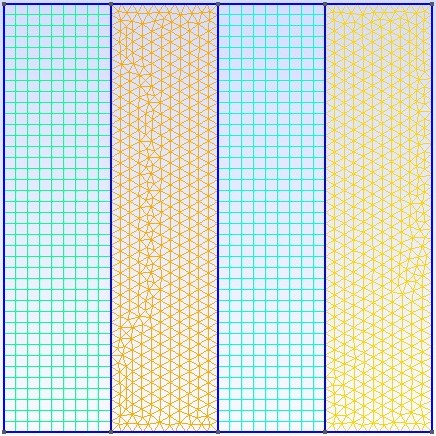
\includegraphics[width=0.4\linewidth, align=c]{HW3/2Structured2furious.jpg} Figure 2 & {[0.0073479]} & {[0.0697943]}\\
        
\includegraphics[width=0.4\linewidth, align=c]{HW3/minikt.jpeg} Figure 3 & {[0.0]} & {[0.0]}\\
        
\includegraphics[width=0.4\linewidth, align=c]{HW3/miniks.jpeg} Figure 4 & {[0.0]} & {[0.0]}\\
    \end{tblr}
    }
    \caption{Results for Given Function with Field 1 Dirichlet}
\end{table}
\vspace{-0.5cm}
\begin{table}[H]
    \renewcommand\baselinestretch{1.1}\selectfont
    \centering
    \mbox{}\clap{
    \begin{tblr}
        []{
        rowsep =1mm,
        colspec = {Q[c,m, 2cm]Q[c,m,4.7cm]Q[c,m,4.7cm]},
        vlines, hlines,
        row{1} = {gray9}
        }
        Mesh & Norm (Upwind) & Norm (Rusanov) \\
        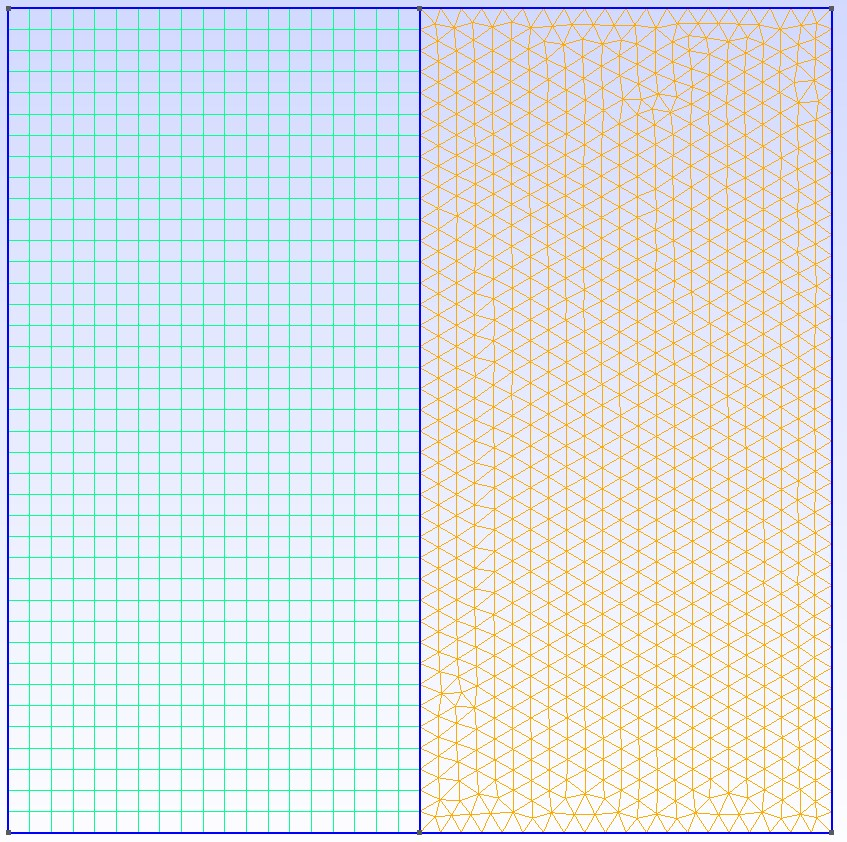
\includegraphics[width=0.4\linewidth, align=c]{HW3/Test Mesh Provided.jpg} Figure 1 & {[-0.0015359]} & {[-0.0015359]}\\
        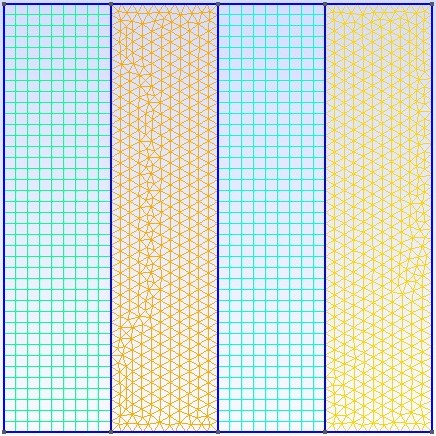
\includegraphics[width=0.4\linewidth, align=c]{HW3/2Structured2furious.jpg} Figure 2 & {[0.0195493]} & {[0.0195493]}\\
        
\includegraphics[width=0.4\linewidth, align=c]{HW3/minikt.jpeg} Figure 3 & {[-0.0005196]} & {[-0.0005196]}\\
        
\includegraphics[width=0.4\linewidth, align=c]{HW3/miniks.jpeg} Figure 4 & {[0.0]} & {[0.0]}\\
    \end{tblr}
    }
    \caption{Results for Given Function with Field 2 Dirichlet}
\end{table}
\begin{table}[H]
    \renewcommand\baselinestretch{1.1}\selectfont
    \centering
    \mbox{}\clap{
    \begin{tblr}
        []{
        rowsep =1mm,
        colspec = {Q[c,m, 2cm]Q[c,m,4.7cm]Q[c,m,4.7cm]},
        vlines, hlines,
        row{1} = {gray9}
        }
        Mesh & Norm (Upwind) & Norm (Rusanov) \\
        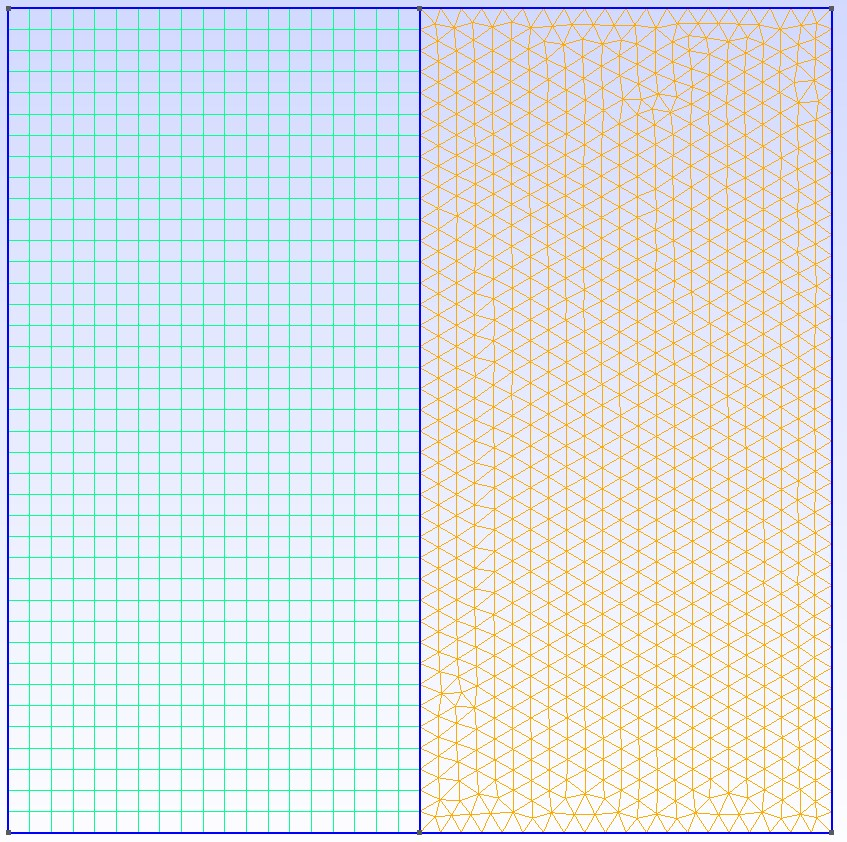
\includegraphics[width=0.4\linewidth, align=c]{HW3/Test Mesh Provided.jpg} Figure 1 & {[0.0060644]} & {[0.0060644]}\\
        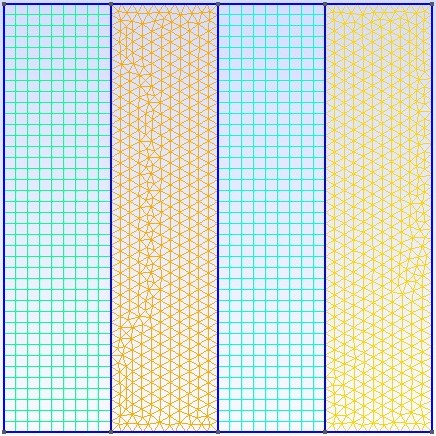
\includegraphics[width=0.4\linewidth, align=c]{HW3/2Structured2furious.jpg} Figure 2 & {[0.0309567]} & {[0.0309567]}\\
        
\includegraphics[width=0.4\linewidth, align=c]{HW3/minikt.jpeg} Figure 3 & {[0.0000127]} & {[0.0000127]}\\
        
\includegraphics[width=0.4\linewidth, align=c]{HW3/miniks.jpeg} Figure 4 & {[0.0008162]} & {[0.0008162]}\\
    \end{tblr}
    }
    \caption{Results for Given Function with Field 3 Dirichlet}
\end{table}
\vspace{-0.5cm}
\subsubsection{Timestep = 1.0}
\vspace{-0.5cm}
\begin{table}[H]
    \renewcommand\baselinestretch{1.1}\selectfont
    \centering
    \mbox{}\clap{
    \begin{tblr}
        []{
        rowsep =1mm,
        colspec = {Q[c,m, 2cm]Q[c,m,4.7cm]Q[c,m,4.7cm]},
        vlines, hlines,
        row{1} = {gray9}
        }
        Mesh & Norm (Upwind) & Norm (Rusanov) \\
        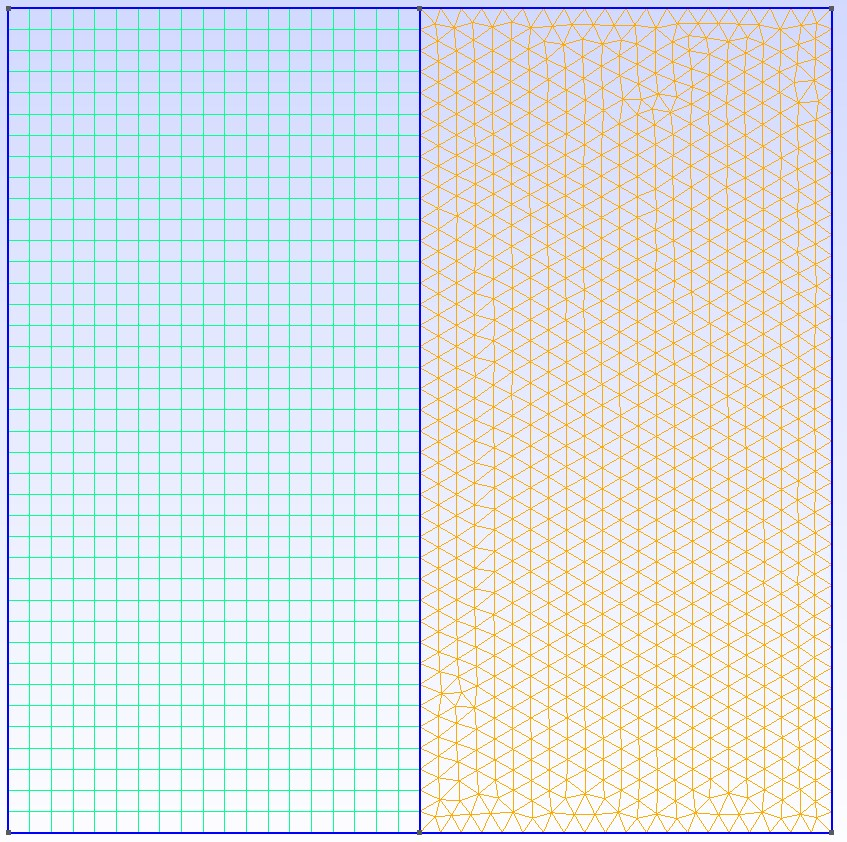
\includegraphics[width=0.4\linewidth, align=c]{HW3/Test Mesh Provided.jpg} Figure 1 & {[0.0018640]} & {[0.0018640]}\\
        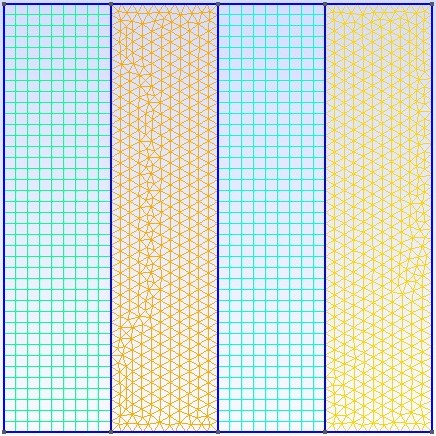
\includegraphics[width=0.4\linewidth, align=c]{HW3/2Structured2furious.jpg} Figure 2 & {[0.0073479]} & {[0.0073479]}\\
        
\includegraphics[width=0.4\linewidth, align=c]{HW3/minikt.jpeg} Figure 3 & {[0.0]} & {[0.0]}\\
        
\includegraphics[width=0.4\linewidth, align=c]{HW3/miniks.jpeg} Figure 4 & {[0.0001020]} & {[0.0001020]}\\
    \end{tblr}
    }
    \caption{Results for Given Function with Field 1 Dirichlet}
\end{table}
\vspace{-0.5cm}
\begin{table}[H]
    \renewcommand\baselinestretch{1.1}\selectfont
    \centering
    \mbox{}\clap{
    \begin{tblr}
        []{
        rowsep =1mm,
        colspec = {Q[c,m, 2cm]Q[c,m,4.7cm]Q[c,m,4.7cm]},
        vlines, hlines,
        row{1} = {gray9}
        }
        Mesh & Norm (Upwind) & Norm (Rusanov) \\
        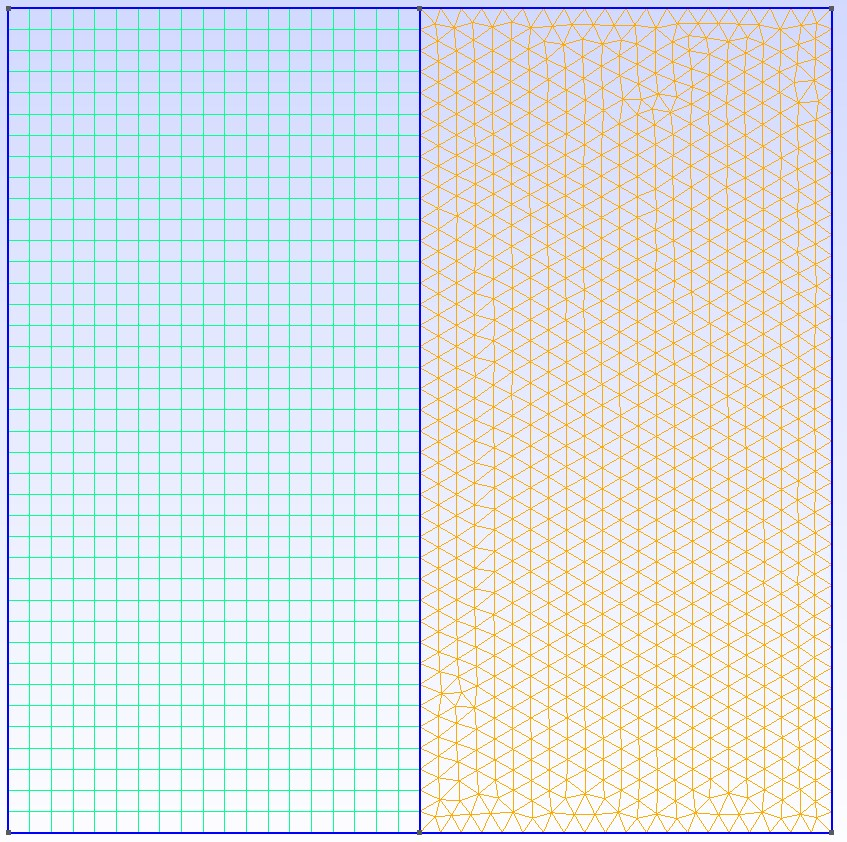
\includegraphics[width=0.4\linewidth, align=c]{HW3/Test Mesh Provided.jpg} Figure 1 & {[-0.0055753]} & {[-0.0055753]}\\
        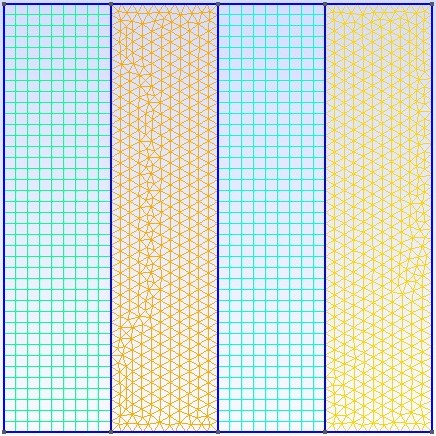
\includegraphics[width=0.4\linewidth, align=c]{HW3/2Structured2furious.jpg} Figure 2 & {[0.0222544]} & {[0.0222544]}\\
        
\includegraphics[width=0.4\linewidth, align=c]{HW3/minikt.jpeg} Figure 3 & {[-0.0006928]} & {[-0.0006928]}\\
        
\includegraphics[width=0.4\linewidth, align=c]{HW3/miniks.jpeg} Figure 4 & {[0.0]} & {[0.0]}\\
    \end{tblr}
    }
    \caption{Results for Given Function with Field 2 Dirichlet}
\end{table}
\begin{table}[H]
    \renewcommand\baselinestretch{1.1}\selectfont
    \centering
    \mbox{}\clap{
    \begin{tblr}
        []{
        rowsep =1mm,
        colspec = {Q[c,m, 2cm]Q[c,m,4.7cm]Q[c,m,4.7cm]},
        vlines, hlines,
        row{1} = {gray9}
        }
        Mesh & Norm (Upwind) & Norm (Rusanov) \\
        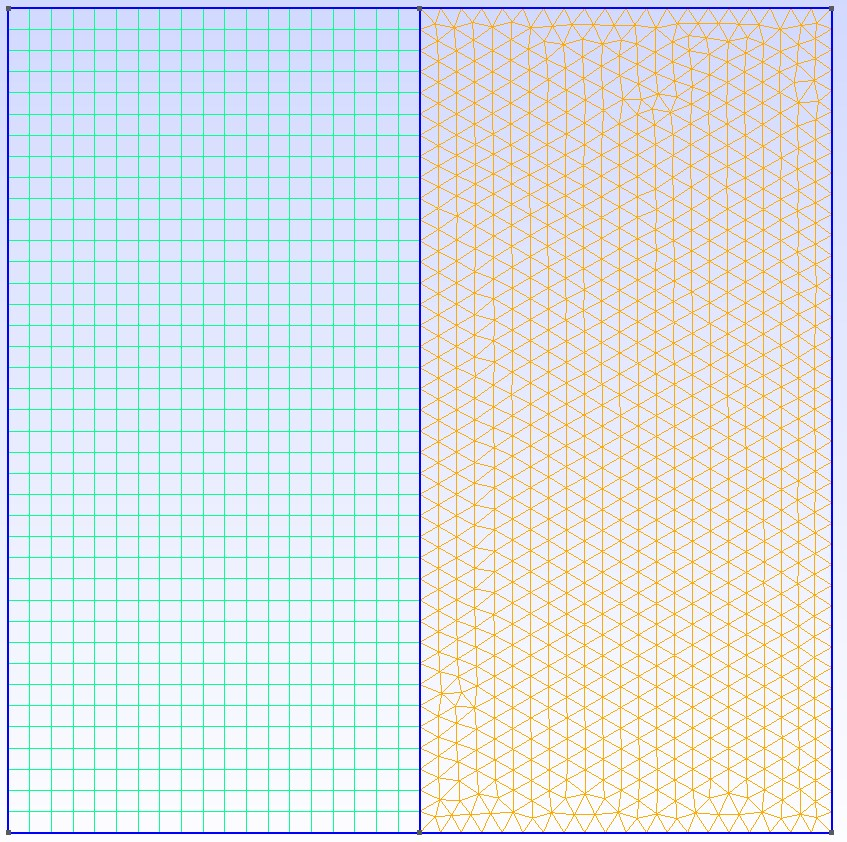
\includegraphics[width=0.4\linewidth, align=c]{HW3/Test Mesh Provided.jpg} Figure 1 & {[0.0092314]} & {[0.0092314]}\\
        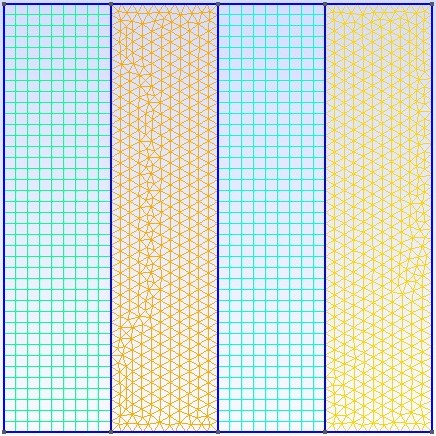
\includegraphics[width=0.4\linewidth, align=c]{HW3/2Structured2furious.jpg} Figure 2 & {[0.0697943]} & {[0.0212781]}\\
        
\includegraphics[width=0.4\linewidth, align=c]{HW3/minikt.jpeg} Figure 3 & {[0.0001917]} & {[0.0001917]}\\
        
\includegraphics[width=0.4\linewidth, align=c]{HW3/miniks.jpeg} Figure 4 & {[0.0007142]} & {[0.0007142]}\\
    \end{tblr}
    }
    \caption{Results for Given Function with Field 3 Dirichlet}
\end{table}
\subsubsection{Modifications to the Function}

To modify the function the \verb|r| value and the \verb|yc| values are adjusted in the \verb|advection.ini| file. All the calculations are ran for a time step of 1.0 and the given velocity field (\hyperref[f1]{\textit{Field 1}}) for simplicity.
\begin{table}[H]
    \renewcommand\baselinestretch{1.1}\selectfont
    \centering
    \mbox{}\clap{
    \begin{tblr}
        []{
        rowsep =1mm,
        colspec = {Q[c,m, 2cm]Q[c,m,4.7cm]Q[c,m,4.7cm]},
        vlines, hlines,
        row{1} = {gray9}
        }
        Mesh & Norm (Upwind) & Norm (Rusanov) \\
        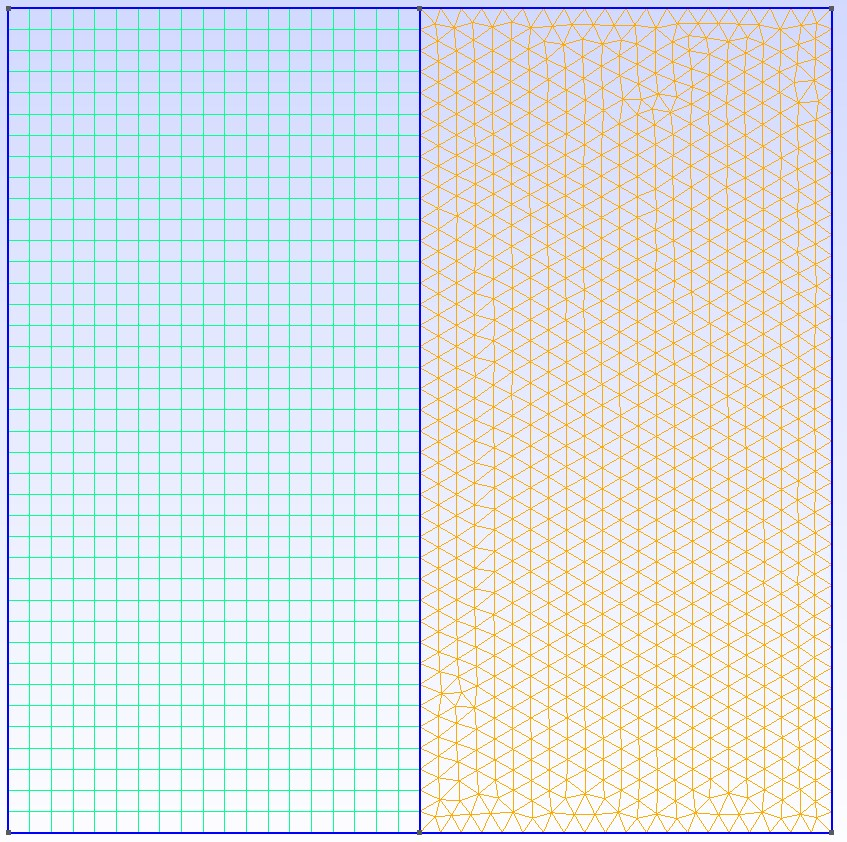
\includegraphics[width=0.4\linewidth, align=c]{HW3/Test Mesh Provided.jpg} Figure 1 & {[-0.0034597]} & {[-0.0034597]}\\
        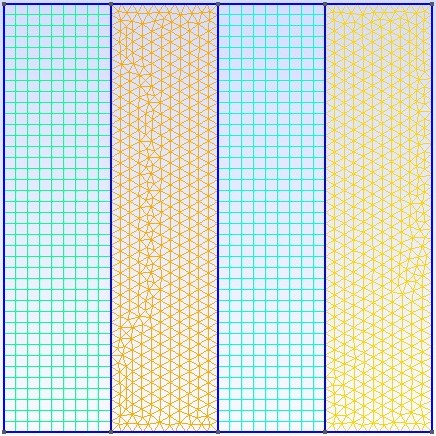
\includegraphics[width=0.4\linewidth, align=c]{HW3/2Structured2furious.jpg} Figure 2 & {[-0.0042726]} & {[-0.0042726]}\\
        
\includegraphics[width=0.4\linewidth, align=c]{HW3/minikt.jpeg} Figure 3 & {[0.0010392]} & {[0.0010392]}\\
        
\includegraphics[width=0.4\linewidth, align=c]{HW3/miniks.jpeg} Figure 4 & {[0.0005101]} & {[0.0005101]}\\
    \end{tblr}
    }
    \caption{Results for $r = 0.05$ with Field 1 Dirichlet}
\end{table} \par
This value alters the region of influence. One would expect a more present value change between the two types, however, due to the lack of quality of the meshes, the difference is not too noticeable. 
\begin{table}[H]
    \renewcommand\baselinestretch{1.1}\selectfont
    \centering
    \mbox{}\clap{
    \begin{tblr}
        []{
        rowsep =1mm,
        colspec = {Q[c,m, 2cm]Q[c,m,4.7cm]Q[c,m,4.7cm]},
        vlines, hlines,
        row{1} = {gray9}
        }
        Mesh & Norm (Upwind) & Norm (Rusanov) \\
        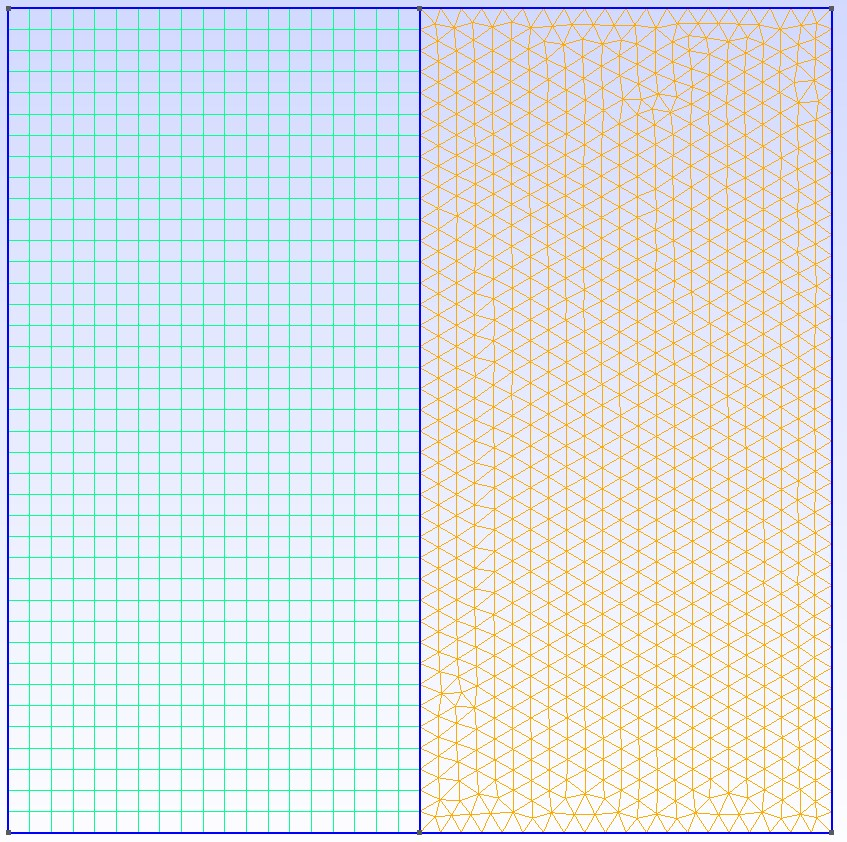
\includegraphics[width=0.4\linewidth, align=c]{HW3/Test Mesh Provided.jpg} Figure 1 & {[0.0]} & {[0.0]}\\
        \includegraphics[width=0.4\linewidth, align=c]{HW3/2Structured2furious.jpg} Figure 2 & {[0.0]} & {[0.0]}\\
        \includegraphics[width=0.4\linewidth, align=c]{HW3/minikt.jpeg} Figure 3 & {[0.0]} & {[0.0]}\\
        \includegraphics[width=0.4\linewidth, align=c]{HW3/miniks.jpeg} Figure 4 & {[0.0]} & {[0.0]}\\
    \end{tblr}
    }
    \caption{Results for $yc = 0.5$ with Field 1 Dirichlet}
\end{table} \par
This value changes the starting location of the influence. For the first two figures due to the interface between the two element types the value changes slightly during operation but as the function rotates due to the purely rotational velocity field the value becomes the same.

\subsection{Comments}

As a first comment about the tests performed, when the results of the Four Section Structured/Unstructured Test Mesh are compared with the provided test mesh, it is clearly seen that the area norms obtained in the provided test mesh are smaller in every case. Another striking trend is the general decrease in the area norms obtained in the Four Section Structured/Unstructured Test Mesh when the time step is reduced. Unfortunately, however, this trend cannot be observed in the results obtained from the tests performed for the provided mesh. In addition, when the tested meshes are examined separately, the area norms calculated depending on the tested velocity fields change significantly in the Four Section Structured/Unstructured Test Mesh. Although similar changes are observed in the provided mesh, the changes as serious as in the Four Section Structured/Unstructured Test Mesh are not observed. \\\par
In addition, when the flux calculation methods were changed from Local-lax Fredric to up-winding scheme, no difference was observed in the calculated area norms.\\\par

The next comment can be obtained by comparing the norms of Field 1 and Field 2 in any flux method, and the mesh type has the lowest area norm since these fields do not interfere with the generic structure of initial conditions. Norms obtained are basically numeric diffusion.\\\par

Another comment is we first expected to see better results for field 1 when the mesh element is triangular and for field 3 when the element type is quadrilateral since it is expected to see advection compatibility of quadrilateral mesh elements is better than triangular counterparts and vice versa for rotating. Yet, the results indicate the exact opposite of this insight. Triangular mesh elements are more suitable for advection motion while \\\par

 The next comment is about field 4. As one can see through the report only three tables were provided for each time step. These tables represent each vector field for that time step. Despite having four vector fields, only three of them have results because of the reason shared previously. The velocity discontinuity at the middle causes the code to fail and therefore there are no results for that vector field.\\\par

Normally, one would expect a bigger difference between the two flux schemes. However, as the meshes are coarse the difference is not noticeable. \\\par

As an added bonus, throughout the code machine epsilon was added to certain equations to prevent division by 0 errors that may arise from truncation and round-off errors.
% BURDA SAĞDA SODLA MACHINE EPLSILON KULLANDIK ZAAA DICEZ


\newpage
\printbibliography
\newpage
\appendix
\section{Mesh Table}
\begin{table}[h]
    \renewcommand\baselinestretch{1.1}\selectfont
    \centering
    \mbox{}\clap{
    \begin{tblr}[]{
        rowsep = 1mm,
        colspec = {Q[c,m, 4.5cm]Q[c,m,3cm]Q[c,m,3cm]Q[c,m,6cm]},
        vlines, hlines,
        row{1} = {gray9}
        }
         Mesh & Element Count & Node Count & Reason \\
         \includegraphics[width=0.63\linewidth, align=c]{HW3/Test Mesh Provided.jpg} Figure 1 & 2782 & 1740 & Default mesh \\
         \includegraphics[width=0.63\linewidth, align=c]{HW3/2Structured2furious.jpg} Figure 2 & 2863 & 1720 & More transition between types \\
         \includegraphics[width=0.63\linewidth, align=c]{HW3/minikt.jpeg} Figure 3 & 6028 & 3013 & A fine triangular grid \\
         \includegraphics[width=0.63\linewidth, align=c]{HW3/miniks.jpeg} Figure 4 & 10201 & 10000 & A fine structured grid \\
    \end{tblr}
    }
    \caption{Statistics of Meshes}
    \label{ap}
\end{table}
\newpage
\section{Velocity Fields}
\begin{table}[h]
    \renewcommand\baselinestretch{1.1}\selectfont
    \centering
    \mbox{}\clap{
    \begin{tblr}
        []{
        rowsep =1mm,
        colspec = {Q[c,m, 5cm]Q[c,m,3cm]Q[c,m,3cm]Q[c,m,3cm]},
        vlines, hlines,
        row{1} = {gray9}
        }
        Field & $u_x$ & $u_y$ & $u_z$  \\
        {\includegraphics[width=0.65\linewidth, align=c]{HW3/default_vel.jpg} Field 1} & {$-2\pi(y-0.5)$} & {$2\pi(x-0.5)$} & {na}\\
        \includegraphics[width=0.65\linewidth, align=c]{HW3/vf2.jpeg} Field 2 & {$sin(\pi x)cos(\pi y)$} & {$-cos(\pi x)sin(\pi y)$} & {na}\\
        \includegraphics[width=0.65\linewidth, align=c]{HW3/vf3.jpeg} Field 2 & {$0.3$} & {$0.0$} & {na}\\
        \includegraphics[width=0.65\linewidth, align=c]{HW3/vf4.jpeg} Field 2 & {$y-0.5$} & {$0.0$} & {na}\\
    \end{tblr}
    }
    \caption{Different Velocity Fields}
    \label{ap2}
\end{table}
\end{document}